\documentclass[12pt]{article}
\usepackage[english]{babel}
\usepackage[utf8x]{inputenc}
\usepackage{amsmath}
\usepackage{tikz}
\usepackage{booktabs}
\usepackage{graphicx}
\usepackage{hyperref}
\usepackage{pdflscape}
\usepackage{adjustbox}
\graphicspath{ {./images/} }
\usepackage{capt-of}
\begin{document}

\begin{titlepage}
\newcommand{\HRule}{\rule{\linewidth}{0.5mm}} 
\center
\textsc{\LARGE SMT. PARVATIBAI CHOWGULE }\\[0.3cm] 
\textsc{\LARGE OF ARTS AND SCIENCE  }\\[0.3cm]
\textsc{\Large GOA-403601, GOA(INDIA) }\\[0.3cm]
\textsc{\Large Computer Science and Engineering}\\[0.5cm] 

\HRule \\[0.4cm] 
{ \huge \bfseries Clustered Machine Learning\par for Predicting Diabetes}\\[0.04cm] 
\HRule \\[1.5cm]

 
\begin{minipage}{0.4\textwidth}
\begin{flushleft} \large
\emph{Submitted By:}\\
Alexander Roque Rodrigues\\SU170331\\TYBSC
\end{flushleft}
\end{minipage}
~
\begin{minipage}{0.4\textwidth}
\begin{flushright} \large
\emph{Submitted To:} \\
Mrs. Ashweta Fondekar\\Asst. Professor\\Dept. of CSE 
\end{flushright}
\end{minipage}\\[1cm]


{\large June-February\\2019-2020 \\Graduation Dissertation}\\[1cm] 


\vfill
\end{titlepage}

\section{Acknowledgements}

\newpage
\tableofcontents
\newpage


\begin{abstract}
Your abstract.
\end{abstract}

\section{Introduction}
In recent days, there has been a sharp increase in the cases of diabetes mellitus. Diabetes mellitus is on the rise amongst many people and the rate of contracting this lifestyle disease could be reduced significantly if proper measures and precautions were to be instilled amongst people the number of people can be reduced.

Machine learning is a growing field in computer science. With the development and introduction of many algorithms the prediction and accuracy of the predictions itself has improved substantially. Machine learning and healthcare systems are also becoming increasingly popular in the healthcare sector.

The project encompasses the qualities of Remote Patient Monitoring (RPM) and Clinical Decision Support (CDS). RPM provides medical facilities that have the ability to transmit patient data to healthcare professionals who might very well be halfway around the world. RPM can monitor blood glucose levels and blood pressure. It is particularly helpful for patients with chronic conditions such as type 2 diabetes, hypertension, or cardiac disease. Data collected and transmitted via PRM can be used by a healthcare professional or a healthcare team to detect medical events such as stroke or heart attack that require immediate and aggressive medical intervention. Data collected may be used as part of a research project or health study. RPM is a life-saving system for patients in remote areas who cannot access face-to-face health care. CDS analyzes data from clinical and administrative systems. The aim is to assist healthcare providers in making informed clinical decisions. Data available can provide information to medical professions who are preparing diagnoses or predicting medical conditions like drug interactions and reactions. CDS tools filter information to assist healthcare professionals in caring for individual clients. 

The objective of this project is to create a  system that is able to use the machine learning algorithms and predict the outcome of the parameters entered into the algorithm and help the patient draw a conclusion whether or not he/she has the same traits exibhited by simillar patients that have diabetes. Also the system should have a UI that is capable of displaying the data of the patients to the doctor and to the patients themselves for further interpretation.

\newpage
\section{System Specifications and Requirements}
The main function of this project is to enable the doctors to advise their patients with the help of the prediction software. The system should be accessible to the patient as weel as the doctor, therefore it should have a web interface for the two parties to interact with. 
\subsection{Functionalities for Doctors}
As an owner of a doctors account a doctor should be able to:
\begin{itemize}
\item Add new patients.
\item Add new observations for the machine learning algorithm to predict.
\item Analyse the patients previous records.
\item Leave notes for patients to act on.
\end{itemize}
\subsection{Functionalities for Patients}
As the patient, one should be able to:
\begin{itemize}
\item Should be able to see the predicted risk of developing diabetes.
\item Should be 
\end{itemize}



\tikzset{every picture/.style={line width=0.75pt}} %set default line width to 0.75pt        

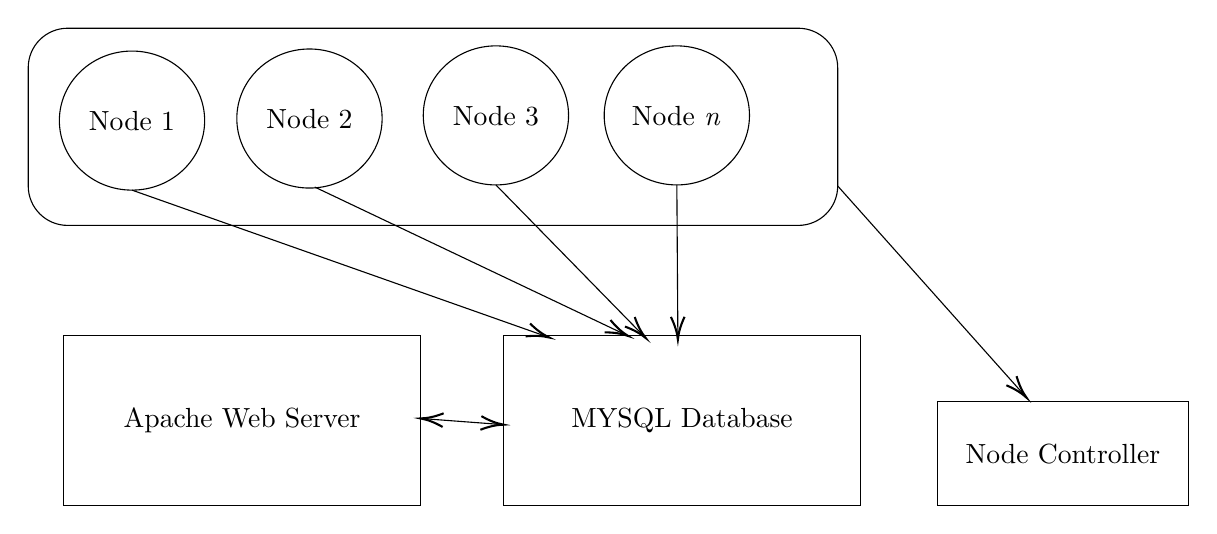
\begin{tikzpicture}[x=0.75pt,y=0.75pt,yscale=-1,xscale=1]
%\path (0,300); %set diagram left start at 0, and has height of 300

%Shape: Ellipse [id:dp750257553390336] 
\draw   (126.5,66.5) .. controls (126.5,48) and (142.17,33) .. (161.5,33) .. controls (180.83,33) and (196.5,48) .. (196.5,66.5) .. controls (196.5,85) and (180.83,100) .. (161.5,100) .. controls (142.17,100) and (126.5,85) .. (126.5,66.5) -- cycle ;
%Shape: Ellipse [id:dp5517632931366927] 
\draw   (41,67.5) .. controls (41,49) and (56.67,34) .. (76,34) .. controls (95.33,34) and (111,49) .. (111,67.5) .. controls (111,86) and (95.33,101) .. (76,101) .. controls (56.67,101) and (41,86) .. (41,67.5) -- cycle ;
%Shape: Ellipse [id:dp5374080086888451] 
\draw   (303.5,65) .. controls (303.5,46.5) and (319.17,31.5) .. (338.5,31.5) .. controls (357.83,31.5) and (373.5,46.5) .. (373.5,65) .. controls (373.5,83.5) and (357.83,98.5) .. (338.5,98.5) .. controls (319.17,98.5) and (303.5,83.5) .. (303.5,65) -- cycle ;
%Shape: Ellipse [id:dp8044448361556924] 
\draw   (216.33,65) .. controls (216.33,46.5) and (232,31.5) .. (251.33,31.5) .. controls (270.66,31.5) and (286.33,46.5) .. (286.33,65) .. controls (286.33,83.5) and (270.66,98.5) .. (251.33,98.5) .. controls (232,98.5) and (216.33,83.5) .. (216.33,65) -- cycle ;
%Shape: Rectangle [id:dp8321414581757052] 
\draw   (43,171) -- (215,171) -- (215,253) -- (43,253) -- cycle ;
%Shape: Rectangle [id:dp7881290703605675] 
\draw   (255,171) -- (427,171) -- (427,253) -- (255,253) -- cycle ;
%Shape: Rectangle [id:dp08712722738328926] 
\draw   (464,203) -- (585,203) -- (585,253) -- (464,253) -- cycle ;
%Straight Lines [id:da9361290207986972] 
\draw    (338.5,98.5) -- (338.99,171) ;
\draw [shift={(339,173)}, rotate = 269.62] [color={rgb, 255:red, 0; green, 0; blue, 0 }  ][line width=0.75]    (10.93,-3.29) .. controls (6.95,-1.4) and (3.31,-0.3) .. (0,0) .. controls (3.31,0.3) and (6.95,1.4) .. (10.93,3.29)   ;

%Straight Lines [id:da034185981319537095] 
\draw    (251.33,98.5) -- (322.1,170.82) ;
\draw [shift={(323.5,172.25)}, rotate = 225.62] [color={rgb, 255:red, 0; green, 0; blue, 0 }  ][line width=0.75]    (10.93,-3.29) .. controls (6.95,-1.4) and (3.31,-0.3) .. (0,0) .. controls (3.31,0.3) and (6.95,1.4) .. (10.93,3.29)   ;

%Shape: Boxed Line [id:dp8352925219440996] 
\draw    (164,99.5) -- (313.19,170.39) ;
\draw [shift={(315,171.25)}, rotate = 205.42000000000002] [color={rgb, 255:red, 0; green, 0; blue, 0 }  ][line width=0.75]    (10.93,-3.29) .. controls (6.95,-1.4) and (3.31,-0.3) .. (0,0) .. controls (3.31,0.3) and (6.95,1.4) .. (10.93,3.29)   ;

%Straight Lines [id:da2289673137743029] 
\draw    (76,101) -- (275.11,171.33) ;
\draw [shift={(277,172)}, rotate = 199.45] [color={rgb, 255:red, 0; green, 0; blue, 0 }  ][line width=0.75]    (10.93,-3.29) .. controls (6.95,-1.4) and (3.31,-0.3) .. (0,0) .. controls (3.31,0.3) and (6.95,1.4) .. (10.93,3.29)   ;

%Straight Lines [id:da6645084801724916] 
\draw    (216.99,211.15) -- (253.01,213.85) ;
\draw [shift={(255,214)}, rotate = 184.29] [color={rgb, 255:red, 0; green, 0; blue, 0 }  ][line width=0.75]    (10.93,-3.29) .. controls (6.95,-1.4) and (3.31,-0.3) .. (0,0) .. controls (3.31,0.3) and (6.95,1.4) .. (10.93,3.29)   ;
\draw [shift={(215,211)}, rotate = 4.29] [color={rgb, 255:red, 0; green, 0; blue, 0 }  ][line width=0.75]    (10.93,-3.29) .. controls (6.95,-1.4) and (3.31,-0.3) .. (0,0) .. controls (3.31,0.3) and (6.95,1.4) .. (10.93,3.29)   ;
%Rounded Rect [id:dp5843838457473232] 
\draw   (26,42) .. controls (26,31.51) and (34.51,23) .. (45,23) -- (397,23) .. controls (407.49,23) and (416,31.51) .. (416,42) -- (416,99) .. controls (416,109.49) and (407.49,118) .. (397,118) -- (45,118) .. controls (34.51,118) and (26,109.49) .. (26,99) -- cycle ;
%Straight Lines [id:da9697808233726559] 
\draw    (416,99) -- (505.67,199.51) ;
\draw [shift={(507,201)}, rotate = 228.26] [color={rgb, 255:red, 0; green, 0; blue, 0 }  ][line width=0.75]    (10.93,-3.29) .. controls (6.95,-1.4) and (3.31,-0.3) .. (0,0) .. controls (3.31,0.3) and (6.95,1.4) .. (10.93,3.29)   ;


% Text Node
\draw (76,67.5) node   [align=left] {Node 1};
% Text Node
\draw (161.5,66.5) node   [align=left] {Node 2};
% Text Node
\draw (251.33,65) node   [align=left] {Node 3};
% Text Node
\draw (338.5,65) node   [align=left] {Node \textit{n}};
% Text Node
\draw (129,212) node   [align=left] {Apache Web Server};
% Text Node
\draw (341,212) node   [align=left] {MYSQL Database};
% Text Node
\draw (524.5,228) node   [align=left] {Node Controller};
\end{tikzpicture}

\newpage
\section{Finding the Right Algorithm}
For our predictions we need to use algorithms that give us the maximum accuracy and once we find that algorithm we will further need to tune the selected algorithm from the algorithms we selected to optimise the performance of the predictions generated by the machine learning algorithm. For this purpose we turn to the EDA or exploratory data analysis stage of any machine learning project. 

\section{Components and Frameworks}

%https://www.scott-clark.com/2018/10/01/types-of-information-systems-used-in-healthcare-facilities/
\newpage
\bibliography{bib}
\end{document}